\chapter{Database Design}

\section{Entities, Attributes and Relationships}
The database, called rokers, will have five tables, songs, albums, artits, playlists, songArtist. Each will hold information about songs and the artistis and other important details. The two
tables will be linked through a foreign key. The student table has the following fields:\\
\begin{figure}[H]
\centering


\section{ER Schema}
\begin{figure}[H]
\centering
\caption{Entity Relationship Diagram}
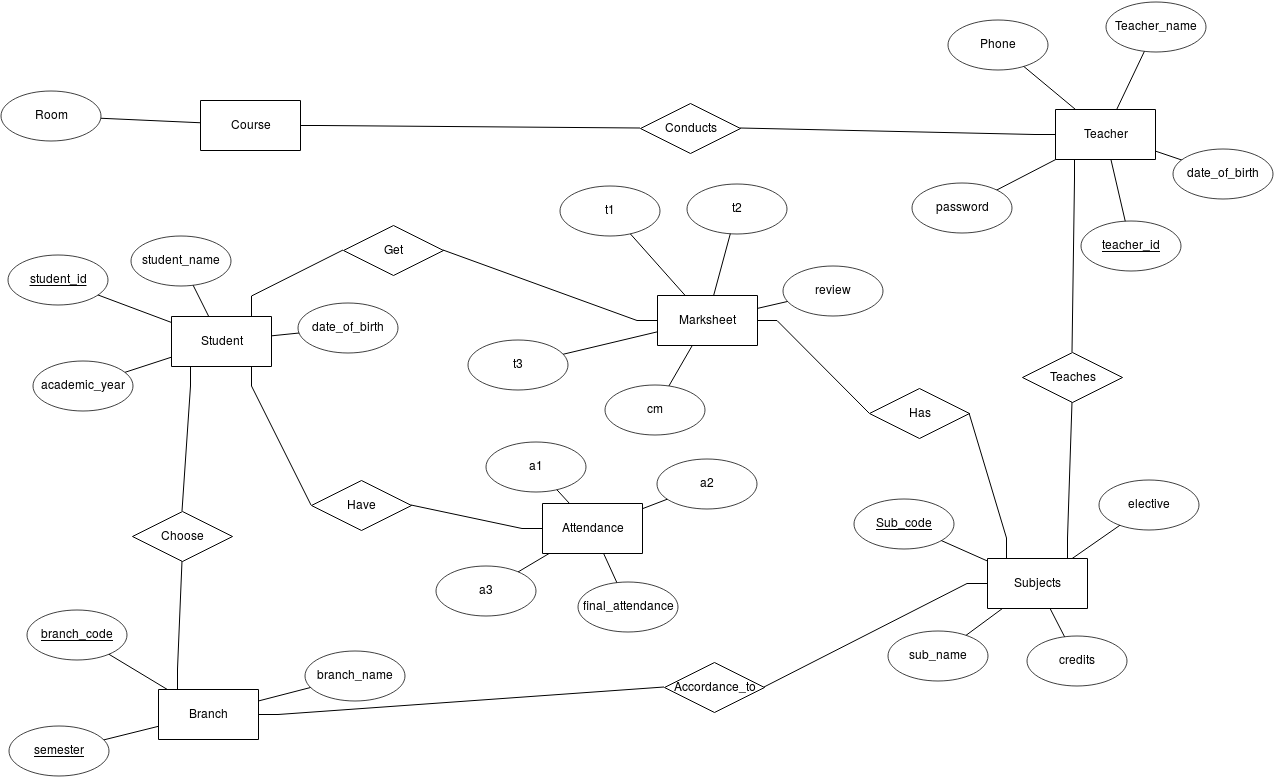
\includegraphics[width=\textwidth,height=\textheight,keepaspectratio]{./erd.png}
\\[0.2in]
\label{fig:Entitiy Relationship Diagram}
\end{figure}

\pagebreak
\thispagestyle{fancy}

\section{Schema Diagram}
\begin{figure}[H]
\centering
\caption{Relational Schema}
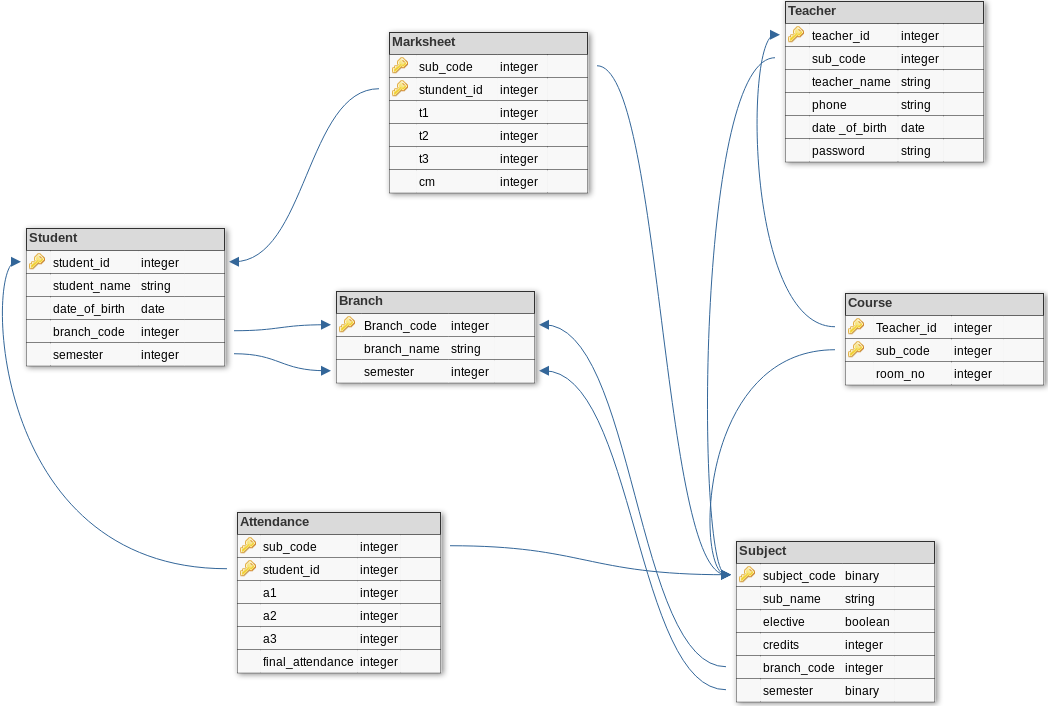
\includegraphics[scale=.5]{./schema.png}
\\[0.2in]
\label{fig:Relational Schema}
\end{figure}

\thispagestyle{fancy}